% !TeX root = ../main_editorial.tex
\documentclass[../main_editorial.tex]{subfiles} % Inherits definitions from parent .tex file.

% Per-problem variable definitions
\newcommand{\problemName}{Sirkus Keliling}
\newcommand{\problemWriter}{Pusaka Kaleb Setyabudi}
\newcommand{\problemEditorialWriter}{Pusaka Kaleb Setyabudi}
\newcommand{\problemTags}{\textit{min-cost max flow}}

\tikzset{
	EdgeStyle/.append style = {->, pos=0.7} }

\begin{document}

\begin{center}
    \section*{\problemName}
    \addcontentsline{toc}{section}{\problemName} % for pdf indexing
    
    \begin{tabular}{rl}
    Penulis soal : & \problemWriter \\
    Penulis editorial : & \problemEditorialWriter \\
    Tema : & \problemTags
    \end{tabular}
\end{center}

\subsection*{Catatan/Komentar}
\addcontentsline{toc}{subsection}{Catatan/Komentar} % for pdf indexing

Batasan yang berlaku pada versi mudah dan sulit:

\begin{itemize}
	\item 1 $ \leq $ T $ \leq $ 5
	\item 1 $ \leq $ M $ \leq $ N $ \times $ (N - 1)
	\item 1 $ \le $ S[i], W[i] $ \le $ 8.000.000
	\item 1 $ \le $ U[i], V[i] $ \le $ N
	\item U[i] $ \neq $ V[i]
	\item (U[i], V[i]) $ \neq $ (U[j], V[j]) untuk i $ \neq $ j
\end{itemize}

Trivia: Soal ini pada awalnya berjudul ``Trayek Bis'' dengan tema penentuan trayek-trayek transportasi. Namun, karena hal ``trayek yang menghubungkan satu kota dengan dirinya sendiri'' dianggap terlalu \textit{absurd}, maka diganti dengan tema yang dipakai saat ini.

\subsection*{Versi Mudah}
\addcontentsline{toc}{subsection}{Versi Mudah} % for pdf indexing
Batasan: $ 1 \le N \le 12 $

Karena batasan nilai $ N $ yang cukup kecil, penyelesaian versi mudah dapat dilakukan dengan menggunakan \textit{Dynamic Programming} dengan teknik \textit{bitmask} sebagai berikut.

Didefinisikan dua buah fungsi berikut:

\begin{enumerate}
	\item $ f(u, C, s) $ dengan $ 1 \le u, s \le N $, $ C \subseteq \{1, 2, \mathellipsis, N\} \backslash \{u, s\} $, yang menyatakan biaya untuk memanfaatkan sirkus keliling yang dimulai dari kota $ s $ untuk mengunjungi kota-kota $ C $ dengan keadaan telah mencapai kota $ u $.
	\item $ g(K) $ dengan $ K \subseteq \{1, 2, \mathellipsis, N\} $, yang menyatakan biaya untuk menentukan pemanfaatan sirkus keliling dan sirkus lokal untuk kota-kota $ K $.
\end{enumerate}

Untuk fungsi DP pertama, rekurensi dapat dilakukan serupa dengan rekurensi pada penyelesaian DP untuk permasalahan \textit{traveling salesman problem}\footnote{dapat mengacu pada halaman ini: \href{http://www.geeksforgeeks.org/travelling-salesman-problem-set-1/}{http://www.geeksforgeeks.org/travelling-salesman-problem-set-1/}} yang memiliki kompleksitas $ \bigO{N^2 \cdot 2^N} $.

Untuk fungsi DP kedua, rekurensinya dapat didefinisikan sebagai berikut.

$$
g(K) = 
\begin{cases}
	0, & K = \emptyset \\
	\displaystyle \min_{\substack{K'\subseteq K \\ K' \neq \emptyset \\ u \in K'}}{\left(f\left(u, K' - \{u\}, u\right) + g\left(K - K'\right)\right)}, & K \neq \emptyset
\end{cases}
$$

Perhatikan bahwa pada rekurensi di atas, pencarian $ K' \subseteq K $ dapat dilakukan dalam kompleksitas $ \bigO{3^N} $.

Kompleksitas akhir dari solusi ini adalah $ \bigO{3^N + N^2 \cdot 2^N} $, cukup untuk mendapatkan \textit{accepted} pada versi mudah.

\pagebreak

\subsection*{Versi Sulit}
\addcontentsline{toc}{subsection}{Versi Sulit} % for pdf indexing
Batasan: $ 1 \le N \le 250 $

Solusi untuk versi sulit dapat dicari melalui nilai \textit{min-cost max flow} dari bentuk graf awal yang telah dimodelkan sebagai berikut (sebagai contoh, diambil $ N = 3 $).

\begin{center}
\begin{tikzpicture}

\Vertex[L=$ 1_{out} $, x=0, y=2]{1}
\Vertex[L=$ 1_{in} $, x=4, y=4]{1'}
\Vertex[L=$ 2_{out} $, x=0, y=0]{2}
\Vertex[L=$ 2_{in} $, x=4, y=0]{2'}
\Vertex[L=$ 3_{out} $, x=0, y=-2]{3}
\Vertex[L=$ 3_{in} $, x=4, y=-4]{3'}

\Edge[label = $ s_1 $](1)(1')
\Edge[label = $ s_2 $](2)(2')
\Edge[label = $ s_3 $](3)(3')

\Edge[label = $ c_{1, 2} $](1)(2')
\Edge[label = $ c_{1, 3} $](1)(3')
\Edge[label = $ c_{2, 1} $](2)(1')
\Edge[label = $ c_{2, 3} $](2)(3')
\Edge[label = $ c_{3, 1} $](3)(1')
\Edge[label = $ c_{3, 2} $](3)(2')

\end{tikzpicture}
\end{center}

Dalam bentuk tersebut, setiap \textit{node} pada soal dipecah menjadi dua bagian, yaitu \textit{node} yang harus tepat memiliki \textit{outdegree} tepat 1 dan \textit{node} yang harus tepat memiliki \textit{indegree} tepat 1. Dengan demikian, setiap \textit{node} harus dipasangkan antara dengan dirinya sendiri (\textit{outdegree} dan \textit{indegree} dari \textit{node} tersebut dipakai untuk membuat suatu \textit{loop}) atau dengan satu \textit{node} lain yang nantinya akan membentuk suatu \textit{cycle} (bayangkan bahwa pada \textit{cycle} terdapat $ n $ \textit{node} dengan \textit{node} pertama ``memakai'' \textit{outdegree}-nya untuk \textit{indegree} dari \textit{node} kedua, \textit{node} kedua ``memakai'' \textit{outdegree}-nya untuk \textit{indegree} dari \textit{node} ketiga, dan seterusnya). Perhatikan bahwa pada solusi di atas, definisi ``memanfaatkan sirkus lokal'' pada suatu kota $ u $ diubah menjadi ``membuat suatu \textit{self-loop}'' pada kota $ u $ dengan biaya sebesar $ s_u $.

Eksekusi algoritma \textit{min-cost max flow} pada graf tersebut akan memastikan bahwa setiap \textit{node} dalam soal akan terpasangkan pada (1) dirinya sendiri (melalui \textit{edge} dengan \textit{cost} sebesar $ s_i $) atau (2) \textit{node} lain dengan \textit{cost} sebesar $ c_{i, j} $. Beberapa algoritma yang dapat digunakan adalah modifikasi algoritma Edmonds-Karp atau dapat juga menggunakan algoritma Kuhn-Munkres (Hungarian Algorithm). Modifikasi dari algoritma Edmonds-Karp memiliki kompleksitas $ \bigO{N^3\cdot \log{N}} $ dan algoritma Kuhn-Munkres memiliki kompleksitas $ \bigO{N^3} $. Keduanya mampu mendapatkan \textit{accepted} pada versi sulit dari soal ini.

\end{document}